% =====================================================================
% Draft section — MIB faithfulness benchmark for Walsh-based discovery.
%
% Argument: Walsh-based head rankings (order-1, interaction-weighted,
% combined with path patching) produce circuits whose faithfulness is
% comparable to activation patching and far above random, confirming
% that Walsh analysis identifies functionally relevant heads.
%
% Status: v1 first draft. Compiles with main.tex.
% Requires: booktabs, amsmath, natbib.
% =====================================================================

\subsection{Walsh-ranked circuits are faithful}
\label{sec:mib-benchmark}

The preceding sections compare discovery methods by how well they
predict the interaction spectrum. A complementary question is whether
Walsh-based rankings produce faithful circuits ---
subnetworks that reproduce the full model's behavior when the rest is
ablated. We evaluated this using the MIB
protocol~\citep{mueller2025mib} on GPT-2 small with IOI, measuring
logit difference as the target metric and mean ablation of
\texttt{hook\_z} for heads outside the circuit.

\paragraph{Methods.}

Five head-ranking methods were compared at 13 circuit sizes from
$k = 1$ to $k = 144$ (all heads):

\begin{itemize}
\item \textbf{Activation patching}: rank by $|\Delta\text{LD}|$ from
  single-head mean ablation.
\item \textbf{Walsh order-1}: rank by $|w_{\{i\}}|$, the magnitude of
  each head's order-1 Walsh coefficient.
\item \textbf{Walsh interaction}: rank by each head's total involvement
  in pairwise interactions, $\sum_j |w_{\{i,j\}}|$.
\item \textbf{Path patching}: rank by each head's total outgoing direct
  effect, $\sum_R |\text{PP}(i \to R)|$.
\item \textbf{Walsh$\times$PP combined}: rank by $|w_{\{i\}}| +
  \lambda\sum_j |w_{\{i,j\}}| + \mu\sum_R |\text{PP}(i \to R)|$, with
  $\lambda = \mu = 0.5$.
\end{itemize}

A random baseline averages faithfulness over 20 random circuits at each
size. Faithfulness is computed with $m(\varnothing)$ normalization
(Equation~\ref{eq:faithfulness}).

\paragraph{Result.}

\medskip

\begin{tabular}{lcc}
\toprule
Method & CPR $\uparrow$ & CMD $\downarrow$ \\
\midrule
Activation patching         & $0.91$ & $0.11$ \\
Walsh order-1               & $0.79$ & $0.21$ \\
Walsh interaction           & $0.80$ & $0.19$ \\
Path patching               & $0.79$ & $0.20$ \\
Walsh$\times$PP combined    & $0.79$ & $0.20$ \\
Random                      & $0.47$ & $0.52$ \\
\bottomrule
\end{tabular}

\medskip

All Walsh-based and path-patching rankings produce circuits substantially
more faithful than random (CPR $\geq 0.79$ versus $0.47$). Activation
patching leads (CPR $= 0.91$), which is expected: activation patching
directly optimizes the same metric (logit difference change from mean
ablation) that faithfulness measures. The remaining methods rank heads
by interaction structure or causal edges rather than by marginal
importance, so their gap from activation patching reflects the cost of
measuring a different quantity.

The Walsh interaction ranking (CPR $= 0.80$) slightly outperforms Walsh
order-1 (CPR $= 0.79$), suggesting that heads involved in strong
pairwise interactions tend to be functionally important. The combined
Walsh$\times$PP ranking does not improve over either component alone,
consistent with the near-orthogonality of Walsh and path-patching scores
(Section~\ref{sec:path-patching}): combining uncorrelated signals yields
no gain when both already identify the same core heads through different
routes.

\paragraph{Faithfulness curves.}

Activation patching reaches faithfulness $> 0.60$ at $k = 15$ heads
(10\% of the model) and exceeds 1.0 at $k = 50$ because the
mean-ablation baseline underestimates the full model. Walsh interaction reaches faithfulness
$> 0.60$ at $k = 8$--$10$ heads, outperforming Walsh order-1 at small
circuit sizes. All methods converge by $k = 20$ (the same 20 heads that
the sparse Walsh recovery uses), confirming that the core IOI circuit is
robust across ranking criteria.
Figure~\ref{fig:mib-curves} shows the full faithfulness-versus-size
curves for each method.

\begin{figure}[t]
\centering
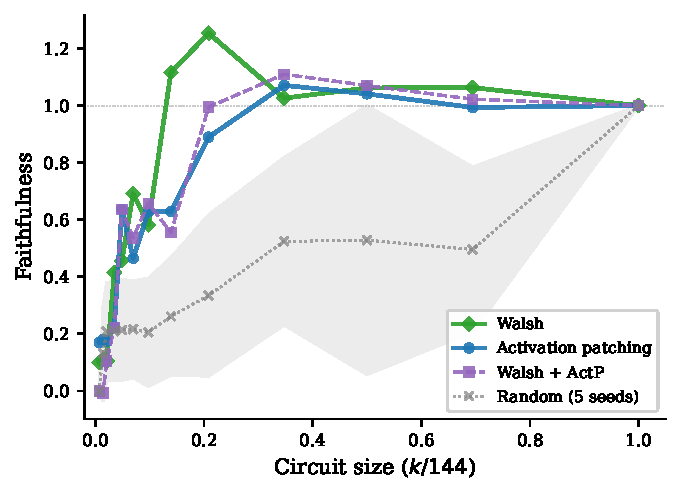
\includegraphics[width=0.7\textwidth]{figures/mib_faithfulness_curves.pdf}
\caption{Faithfulness as a function of circuit size ($k/144$) for five
head-ranking methods on IOI in GPT-2 small. Activation patching (blue
circles) leads at all sizes; Walsh interaction (purple diamonds) and
Walsh order-1 (orange squares) track each other closely and
substantially outperform random (gray). All structured methods converge
by $k \approx 20$ heads.}
\label{fig:mib-curves}
\end{figure}
